% Quiz 7: C, F, the product-rule question, and revised H are selected.
% Solutions: q7-sol-261-II2026.tex. Source notes: q7-shortlist-261-II2026.md.
\documentclass[12pt]{exam}
\usepackage{amsthm}
\usepackage{bm}
\usepackage{libertine}
\usepackage[utf8]{inputenc}
\usepackage[margin=0.5in]{geometry}
\usepackage{amsmath,amssymb}
\usepackage{multicol}
\usepackage[shortlabels]{enumitem}
\usepackage{siunitx}
\usepackage{physics}
\usepackage{booktabs}
\usepackage{graphicx}
\usepackage{pgfplots}
\usepackage{listings}
\usepackage{tikz}
\usepackage{tikz-3dplot}
\usetikzlibrary{arrows.meta,decorations.markings}

\bmdefine{\ii}{i}
\bmdefine{\jj}{j}
\bmdefine{\kk}{k}
\newcommand{\te}{\theta}
\newcommand{\cC}{\mathcal{C}}
\newcommand{\word}[1]{\quad\text{#1}\quad}

\pgfplotsset{width=10cm,compat=1.9}
\usepgfplotslibrary{external}
\tikzexternalize
% Compile the small vector diagram inline, without shell escape.
\tikzexternaldisable

\newcommand{\class}{Math 261-001}
\newcommand{\examnum}{Quiz 7}
\newcommand{\examdate}{October 23}

\begin{document}
\pagestyle{plain}
\thispagestyle{empty}

\noindent
\textbf{\class}\\
\textbf{\examnum}, \textbf{\examdate}

\setlength{\tabcolsep}{3.5cm}
\renewcommand{\arraystretch}{1.5}
\setlength\extrarowheight{1cm}
\begin{tabular}{ |c|c| }
 \hline
 Name   & CSU ID \#  \\
 \hline
\end{tabular}

\vspace{10pt}

Choose and answer \textbf{exactly two} of the four problems. If you attempt
more than two, only the first two will be graded. Write your final answers
in the boxes provided. Only answers in the boxes will be graded.
You may use the surrounding space for scratch work. Each problem is worth
the same number of points.

\begin{enumerate}

% Selected shortlist C, unchanged mathematically.
\item For real constants $a,b$, let
\[
  \vec F_{a,b}(x,y,z)=(2xy+az^2,\ bx^2+z,\ 2xz+y).
\]
Find all pairs $(a,b)$ for which $\vec F_{a,b}$ is conservative.
For those values, find a potential function $f$.

\vfill
\begin{flushright}
\begin{minipage}{0.29\linewidth}
\centering
$(a,b)$\par\smallskip
\framebox(120,50){}
\end{minipage}\hspace{0.4cm}
\begin{minipage}{0.54\linewidth}
\centering
Potential $f(x,y,z)$\par\smallskip
\framebox(250,50){}
\end{minipage}
\end{flushright}

% Selected shortlist F: circulation and outward flux are separate results.
\item Let $\vec F(x,y)=(y^3-2y,\ -4x+3y^2)$, and let $C$ be the
counterclockwise boundary of the rectangle \mbox{$0\leq x\leq2$} and
\mbox{$0\leq y\leq1$}. Find the circulation
$\displaystyle\oint_C\vec F\cdot\vec T\,ds$ and the outward flux
$\displaystyle\oint_C\vec F\cdot\vec N\,ds$, where $\vec T$ is the
unit tangent in the direction of traversal and $\vec N$ is the outward
unit normal.

\vfill
\begin{flushright}
\begin{minipage}{0.46\linewidth}
\centering
Circulation\par\smallskip
\framebox(215,50){}
\end{minipage}\hspace{0.4cm}
\begin{minipage}{0.46\linewidth}
\centering
Outward flux\par\smallskip
\framebox(215,50){}
\end{minipage}
\end{flushright}

\newpage

% Product rule combined with the divergence-of-curl identity.
\item Let
\[
  f(x,y,z)=x^2+y^2+z^2,\qquad \vec G(x,y,z)=(z^2,x^2,y^2).
\]
Compute $\displaystyle\nabla\cdot\bigl(f(\nabla\times\vec G)\bigr)$.

\vfill
\begin{flushright}
\framebox(250,50){}
\end{flushright}

% Revised shortlist H. The quarter-circle center is explicitly (2,0).
\item Use Green's theorem to evaluate $\displaystyle\int_C\vec F\cdot d\vec r$,
where
\[
  \vec F(x,y)=\bigl(ye^{xy}-y,\ xe^{xy}+x+1\bigr).
\]
\noindent\begin{minipage}[c]{0.59\linewidth}
\raggedright
The path $C$ follows, in order, the straight segment
\mbox{$(0,0)\to(3,0)$}, the counterclockwise quarter-circle
$(x-2)^2+y^2=1$ from $(3,0)$ to $(2,1)$, and the straight segment
\mbox{$(2,1)\to(0,1)$}.
\end{minipage}\hfill
\begin{minipage}[c]{0.37\linewidth}
\centering
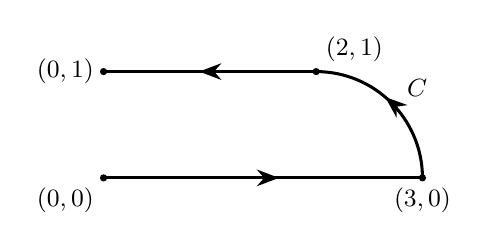
\begin{tikzpicture}[x=1.35cm,y=1.35cm,>=Stealth,
  directed/.style={line width=1.1pt,postaction={decorate},
    decoration={markings,mark=at position 0.55 with {\arrow{Stealth}}}},
  every node/.style={font=\small}]
  % Show only the actual path; no axis suggests the missing closing segment.
  \draw[directed] (0,0) -- (3,0);
  \draw[directed] (3,0) arc[start angle=0,end angle=90,radius=1];
  \draw[directed] (2,1) -- (0,1);
  \fill (0,0) circle (1.3pt) node[below left] {$(0,0)$};
  \fill (3,0) circle (1.3pt) node[below] {$(3,0)$};
  \fill (2,1) circle (1.3pt) node[above right] {$(2,1)$};
  \fill (0,1) circle (1.3pt) node[left] {$(0,1)$};
  \node at (2.95,0.85) {$C$};
\end{tikzpicture}
\end{minipage}

\medskip
\noindent\textit{Reminder:} $\displaystyle\iint_R 1\,dA=\operatorname{Area}(R)$.

\vfill
\begin{flushright}
\framebox(250,50){}
\end{flushright}

\end{enumerate}
\end{document}
